\section{Audio Spectrum Analyzer (ASA)}
\label{sect:ASA}
The AVNA project started with impedance and transmission analysis which is the normal set for a network analyzer.  However, the same hardware is capable of supporting other tests with the only changes being in the firmware.  This leads to a more general descriptor of "Audio Instrument."  One of the resulting instruments is the Spectrum Analyzer, covered here.  Note that, in addition to displaying spectra,  there some specialized tests for the measurement of Signal-to-Noise Ratio and SINAD.  These measurements are covered in this section as well, since they work as part of the Spectrum Analyzer.
\subsection{Description}
\label{subsect:ASADescr}
Within a frequency range of 10 Hz to 40 kHz, the power at the T input terminals is displayed.  Unlike instruments lie the AVNA, the display is graphical with power in dBm (relative to a milliwatt).  The frequency runs along the bottom and is always 0.0 at the left edge and up to 3, 6, 12, 24 or 48 kHz on the right side. 

The dBm calibration assumes an input resistance of 50-Ohms and that resistor should be switch in for the scale reference to be meaningful.  If the input idoes not have the 50-Ohms switched in, it has a 1-Megohm input impedance.  For the high impedance case, the 0 dBM line at the top corresponds to 0.223 V rms or 0.632-V p-p.

The dB per division and the dB offset for the dBm scale can be varied by bottom row menu items.

As will be described in detail below, the spectrum analyzer can also do noise and  distortion measurements.

\subsection{Instructions}
\label{subsect:ASAInstr}
Everything starts with the Instrument Home screen shown in  Figure \ref{AVNA_000-label},  you have a choice of four Audio Test Instruments where for this case we select, "Spectrum Analyzer."  This comes up sweeping with a 48 kHz width displaying an 80 dB range.   This is fine for many purposes and an input can be connected to the T input terminals.  Be careful to not put more than about 1-Volt p-p input.  The ADC will be driven past its range, causing spurious response signals to be displayed, as well as for the proper response to be clipped in amplitude.  At some point, considerably higher, damage can occur to the instrument.

\begin{figure}[H]
\begin{center}
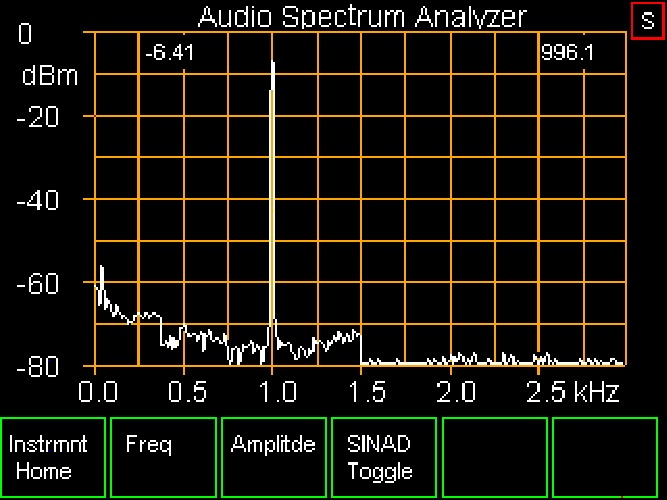
\includegraphics[scale=0.75]{./images/AVNA_019.pdf}
\caption{Spectrum Analyzer  showing a 996 Hz sine wave.  }
\label{AVNA_019-label}
\end{center}
\end{figure}
%
At this point, the screen should look somewhat like that in Figure \ref{AVNA_019-label}.  There will be no spike, as seen at about 1 kHz since there is no signal being applied.  The frequency scale will be different do to adjustments we will discuss in the next paragraph.  It is normal for the noise line to be higher on the left half of the screen and to rise to roughly -50 dBm at the very left edge.

\textbf{Frequency coverage - }To change the frequency range being displayed, we tap on the "Freq" button on the bottom row.  This brings up a screen allowing changes to the maximum frequency and describing parameters  being used.  We have been talking about the maximum display frequency that has been set initially to 48 kHz.  The frequency changing control screen works in terms of "Sample Rate" that is twice the maximum display frequency being displayed.  In addition a parameter, "Maximum Frequency" is shown that is 5/6 of the maximum display frequency.  This is unnecessarily confusing, but reflects that we can only work with inputs up to half of the ADC sampling frequency and further that there is a low-pass filter as part of the ADC that starts cutting off at 5/6 of the sampling frequency.  We show the full frequency range on the display, but we need to remember that the last two divisions on the screen are attenuated and should not be considered as numerically accurate.

So now we can change the total frequency range by adjusting the "Sample Frequency" down with the button on the bottom row.  The first button tap cuts the sample rate in half to 48 kHz.  If we continue tapping this button, we will get to the lowest range with a Sample Frequency of 6 kHz.  This will display 0 to 3 kHz as was seen in Figure  \ref{AVNA_019-label}.  We will later, under Signal Generators, see how to generate a sine wave as seen in the figure.


On the ASA frequency control screen,  we also see a numerical value for the Resolution Bandwidth.  This reflects the sampling rate as well as the 1024 point FFT being used.  In addition, resolution shown includes the 1.5 factor due to the Hann window function that is always used.
%
\footnote{The resolution bandwidth of the FFT without windowing is the sampling rate divided by the number of sampling points per FFT, which in our case is 1024.  Windowing is used to reduce the spurious side signals due to taking a finite sample of the waveform.  See, \linebreak \textbf{\texttt{https://en.wikipedia.org/wiki/Window\_function}}}
%
Note that the FFT only gives 512 data points across the half-sample rate region.  There are 256 pixels available to display the data, so each pixel includes a little more than a single unit of FFT resolution.    The only setting involved with this is the Sample Rate setting and the remainder is automatic.

Finally, on the frequency screen there is provision for changing the amount of data averaging.  The advantage of averaging is to reduce the amount of noise seen on the spectral trace  There are many times when this  increases the accuracy of measurements.  The penalty is slowness in the screen updates.

\textbf{Amplitude control - } The vertical axis, when starting up, covers 80 dB of range with 10 dB per division.  The "Amplitude" button at the bottom of the Spectrum Analyzer screen brings up controls for dB per division (dB/div) and dB offset.  The db/div can be set to 20, 10, 5, or 2.  The offset comes in 5 dB increments and can be used to move the screen display up or down.  In all cases, the scale of dBm on the left axis tracks these changes.

\textbf{Marker annotation - }Still looking at the Spectrum Analyzer screen, Figure  \ref{AVNA_019-label},  observe the "-6.41" notation at the top.  This is a measure, in dBm, of the amplitude of the strongest signal on the screen.  It assumes that the signal being measured is narrow band like the sine wave shown.  Over on the right side is a marking "996.1"  This is the estimated frequency of the same strongest signal using a clever method of interpolating the Hann windowed FFT. 
 %
\footnote{See, "A New Accurate FFT Interpolator for Frequency Estimation," \linebreak \textbf{\texttt{ https://forum.pjrc.com/threads/36358-A-New-Accurate-FFT-Interpolator-for-Frequency-Estimation}}. }
%
For reasonably strong signals, this estimated frequency is superior to conventional frequency counters. The estimate is being made in a fraction of a second, but accurate to around 0.1 Hz.   As you might expect, the accuracy diminishes at low signal-to-noise ratio, but still gives a useful estimate.  

\textbf{SINAD and S/N - }The last button on the main Spectrum Analyzer screen is a toggle that activates, or de-activates, some specialized measurements.  These use the same data as is displayed.  The measurement width is automatically set to 6 kHz (12 kHz sample rate) and the special measurements are made near 1 kHz.  There is no FFT bin centered on 1 kHz, so the nearest bin center of 996 Hz is really the center.  The display now looks like Figure \ref{AVNA_020-label}, but missing the signal.
%
\begin{figure}[H]
\begin{center}
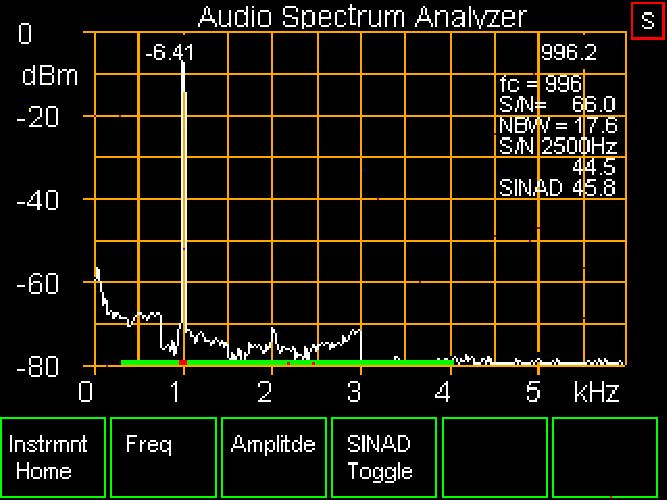
\includegraphics[scale=0.75]{./images/AVNA_020.pdf}
\caption{Spectrum Analyzer screen including SINAD measurements.}
\label{AVNA_020-label}
\end{center}
\end{figure}
%

SINAD is a measurement term that is used primarily to evaluate radio receiver performance.  Rather than trying to cover the definitions and uses of these terms here, please refer to the foot-noted references.
%
\footnote {\textbf{\texttt{https://en.wikipedia.org/wiki/SINAD}}}\textsuperscript{,}
%
\footnote{\textbf{\texttt{https://www.electronics-notes.com/articles/radio/radio-receiver-sensitivity/what-is-sinad-signal-to-noise-and-distortion.php}}}
%
For our ASA, the measurement bandwidth for noise is fixed at 300 to 4000 Hz.  The frequency center, as discussed above, is 996 Hz.  To allow for frequency errors in the signal generator for the 996 Hz tone (this may be an external generator that is part of an RF signal generator), the signal measurement adds 3 FFT bin powers together which is equivalent to a simple band-pass filter of about 40 Hz width, centered on 996 Hz.  The nois plus distortion power measurement excludes 5 bins, or about 60 Hz centered at 994 Hz.

With no signal present, the SINAD should show very close to 0.0 dB.  With increasing signal the SINAD will increase, representing the reduced competition of noise. 

The other measurements shown are "S/N" which is the ratio, in dB, of the power in the signal bins to that in the sum of the two noise bands, scaled back to a single bin bandwidth.   The "NBW"  line is for the calculated Noise Band Width in Hz, and refers to the noise in a single FFT bin (including windowing effects).   The "S/N 2500" is the same as "S/N" except 21.5 dB lower to reflect the wide band.  The reason for posting this tightly coupled number is the popular WSJT series of programs
%
\footnote{\textbf{\texttt{https://physics.princeton.edu/pulsar/k1jt}}}
%
that use this wide band S/N extensively.

\subsection{Discussion}
\label{subsect:ASADiscus}
Multiple FFT are averaged together to produce the ASA graph.  The width of the display can be varied in 2:1 steps from 3 to 48 kHz with the resolution bandwidth varying proportionally.  The normal scale is 80 dB which is10 dB/div, but a 5 dB/div option is available along with offsets in 5 dB steps.  The peak level on the screen is indicated at the top left and the frequency of this peak is at the top right.  The level may be higher than the graphics peak as it is the sum power of the peak "bin" and the two adjacent ones.  The frequency indication includes interpolation between bins and has counter accuracy for stronger sine waves.  The input goes to the right hand Transmission port.  The calibration is in dBm into 50 Ohms and assumes that the 50 Ohm input terminator is switched in.
